%
% Abschlussarbeit mit LaTeX
% ===========================================================================
% This is part of the book "Abschlussarbeit mit LaTeX".
% Copyright (c) 2002-2005 Tobias Erbsland, Andreas Nitsch
% See the file abschlussarbeit_mit_latex.tex for copying conditions.
%

\chapter{Dokumentklassen}
\label{sec:dokumentklassen}
\index{Dokumentklasse}\index{documentclass@\texttt{\textbackslash documentclass}|textbf}

Das grundsätzliche Layout eines \DMLLaTeX"=Dokuments wird durch verschiedene Dokumentklassen bestimmt. Es existieren verschiedenste Pakete, welche weitere Dokumentklassen zu den Standardklassen hinzufügen.

Eine empfehlenswerte Erweiterung von \DMLLaTeX, welche für auch für das vorliegende Dokument verwendet wurde, ist \KOMAScript~\cite{KOMA}\index{KOMA-Script@\KOMAScript}. Wir beschreiben daher von Anfang an den Aufbau mit den \KOMAScript-Klassen. Sie bieten eine Vielzahl von Optionen und einer Anpassung der Standardklassen an die europäische Typographie.

Hier beschreibe ich die drei am häufigsten verwendeten Klassen und die wichtigsten Unterschiede zwischen diesen.

\section{Generelle Syntax, um die Dokumentklasse zu definieren}

Pro Dokument kann nur eine Dokumentklasse definiert werden. Diese Deklaration muss der erste Befehl in deinem \DMLLaTeX"=Dokument, bzw. im Header, sein. Die generelle Syntax, um eine Dokumentklasse zu wählen, ist folgende:
\begin{lstlisting}
\documentclass[Optionen]{Name der Klasse}
\end{lstlisting}

Es existieren dabei verschiedenste Optionen, welche sich auf das Layout des Dokuments auswirken. Sie sind weiter unten im \cref{sec:globaleoptionen} beschrieben und werden auch an alle folgenden \texttt{\textbackslash usepackage}"=Befehle weitergegeben. 

Wenn du bei der Dokumentklasse als Option z.\,B. \enquote{pdftex} angibst, wird diese Option auch an den Befehl \texttt{\textbackslash usepackage\{graphicx\}} weitergegeben. Dort musst du diese Option nicht mehr angeben.
\begin{lstlisting}
\documentclass[Optionen]{Name der Klasse}

\usepackage[Optionen]{Name des Pakets}
\usepackage[Optionen]{Name des Pakets}

\begin{document}
...Dokumentinhalt...
\end{document}
\end{lstlisting}

\section{Globale Optionen}
\label{sec:globaleoptionen}\index{Dokumentklasse!Optionen}

Die nachfolgenden Optionen funktionieren mit den Standardklassen wie auch mit den \KOMAScript-Klassen:

\begin{description}
	\item[10pt, 11pt, 12pt] Wählt die Schriftgröße im Dokument. Standard ist \enquote{10pt}.
	\item[a4paper, a5paper, b5paper, letterpaper, legalpaper]
		Legt das Papier\-format fest. Standard ist \enquote{letterpaper}.
	\item[landscape] Wählt Querformat für das Papier.
	\item[titlepage, notitlepage] Legt fest, ob es eine separate Titelseite
		geben soll oder nicht.
	\item[leqno] Die Nummer bei nummerierten Formeln soll links, statt rechts,
		dargestellt werden.
	\item[fleqn] Formeln sollen linksbündig statt zentriert dargestellt werden.
	\item[openbib] Es soll das \enquote{offene} Bibliographie-Format verwendet werden.
	\item[draft, final] Legt fest, ob es sich bei dem Dokument um einen Entwurf
	  oder um die finale Version handelt. Das wirkt sich auf verschiedene Pakete
	  aus. Beim Entwurf werden z.\,B. Bilder nur als Rahmen dargestellt, und
	  übervolle Boxen werden mit einer Linie markiert.
	\item[oneside, twoside] Wählt, ob die Ausgabe auf doppelseitigem oder auf 
	  einseitigem Papier erfolgen soll.
	\item[openright, openany] Definiert, wo neue Kapitel beginnen dürfen. Mit
		\enquote{openright} werden neue Kapitel nur auf einer rechten Seite begonnen.
	\item[onecolumn, twocolumn] Legt fest, ob der Text ein- oder zweispaltig
		gesetzt werden soll.
\end{description}

Nicht alle Optionen sind bei allen Standardklassen vorhanden. \Cref{tab:classoptions} gibt einen Überblick, welche Optionen bei welchen Klassen vorhanden sind. Dabei zeigt ein \enquote{$\square$}, dass die Option vorhanden ist, und ein \enquote{$\blacksquare$}, dass dies zudem eine voreingestellte Option ist.

\begin{table}[htbp]
	\begin{center}
		\begin{tabular}{r|c|c|c|c|c}
			Optionen $\Downarrow$ Dokumentklassen $\Rightarrow$ &
			\begin{sideways} article \end{sideways} &
			\begin{sideways} report \end{sideways} &
			\begin{sideways} letter \end{sideways} &
			\begin{sideways} book \end{sideways} &
			\begin{sideways} slides \end{sideways}
			\\ \hline
			10pt &
			$\blacksquare$ &
			$\blacksquare$ &
			$\blacksquare$ &
			$\blacksquare$ &
			\\ \hline
			11pt, 12pt &
			$\square$ &
			$\square$ &
			$\square$ &
			$\square$ &
			\\ \hline
			letterpaper &
			$\blacksquare$ &
			$\blacksquare$ &
			$\blacksquare$ &
			$\blacksquare$ &
			$\blacksquare$ \\ \hline
			a4paper, a5paper, b5paper, legalpaper, executivepaper &
			$\square$ &
			$\square$ &
			$\square$ &
			$\square$ &
			$\square$ \\ \hline
			landscape &
			$\square$ &
			$\square$ &
			$\square$ &
			$\square$ &
			$\square$ \\ \hline
			leqno, fleqn &
			$\square$ &
			$\square$ &
			$\square$ &
			$\square$ &
			$\square$ \\ \hline
			openbib &
			$\square$ &
			$\square$ &
			$\square$ &
			$\square$ &
			$\square$ \\ \hline
			final &
			$\blacksquare$ &
			$\blacksquare$ &
			$\blacksquare$ &
			$\blacksquare$ &
			$\blacksquare$ \\ \hline
			draft &
			$\square$ &
			$\square$ &
			$\square$ &
			$\square$ &
			$\square$ \\ \hline
			oneside &
			$\blacksquare$ &
			$\blacksquare$ &
			$\blacksquare$ &
			$\square$ &
			\\ \hline
			twoside &
			$\square$ &
			$\square$ &
			$\square$ &
			$\blacksquare$ &
			\\ \hline
			openany &
			$\blacksquare$ &
			$\blacksquare$ &
			$\blacksquare$ &
			$\square$ &
			\\ \hline
			openright &
			$\square$ &
			$\square$ &
			$\square$ &
			$\blacksquare$ &
			\\ \hline
			onecolumn &
			$\blacksquare$ &
			$\blacksquare$ &
			$\blacksquare$ &
			$\blacksquare$ &
			\\ \hline
			twocolumn &
			$\square$ &
			$\square$ &
			$\square$ &
			$\square$ &
			\\ \hline
			clock & & & & & $\square$ \\
		\end{tabular}
	\end{center}

	\caption{Optionen bei den verschiedenen Standard-Dokumentklassen}
	\label{tab:classoptions}
\end{table}

\section{Dokumentklasse \enquote{scrartcl}}
\index{Dokumentklasse!scrartcl}

\begin{lstlisting}
\documentclass{scrartcl}
\end{lstlisting}

Die Dokumentklasse \enquote{scrartcl} ist für kleine Dokumente gedacht. Dabei wird das Dokument standardmäßig auf einer Seite gesetzt. Der Titel und das Inhaltsverzeichnis folgen einander auf der ersten Seite, direkt gefolgt von dem ersten Abschnitt.

Mögliche Gliederungen in dieser Dokumentklasse sind \texttt{\textbackslash section}, \texttt{\textbackslash subsection},
\\
\texttt{\textbackslash subsubsection}, \texttt{\textbackslash paragraph} und \texttt{\textbackslash subparagraph}.

\Cref{lst:article} erzeugt eine einzelne Seite, so wie sie in \cref{fig:article} zu sehen ist.

\begin{figure}[htb]
	\begin{center}
		\fbox{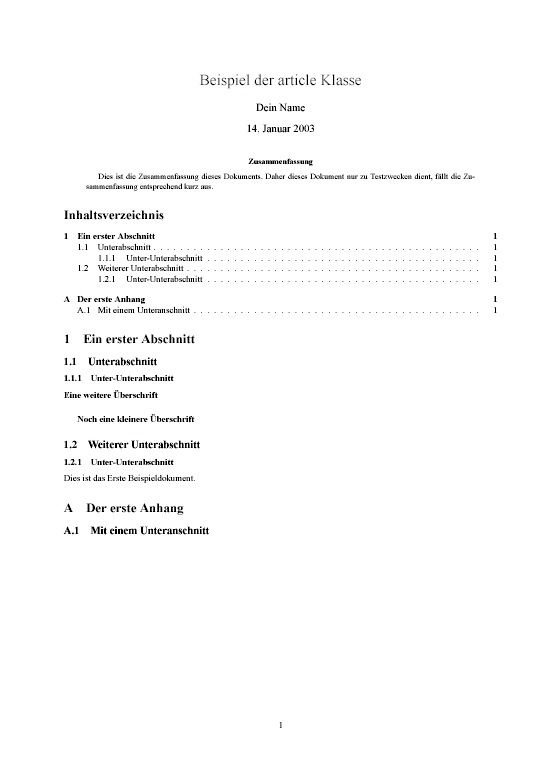
\includegraphics[height=5cm]{images/article_page1.png}}
	\end{center}
	\caption{Aufbau eines Dokuments mit \enquote{scrartcl}}
	\label{fig:article}
\end{figure}

\section{Dokumentklasse \enquote{scrreprt}}
\index{Dokumentklasse!scrreprt}

\begin{lstlisting}
\documentclass{scrreprt}
\end{lstlisting}

Ein \enquote{scrreprt} ist die größere Form eines Dokuments. Das Dokument bekommt eine separate Titelseite, sowie eine separate Seite für die Zusammenfassung und das Inhaltsverzeichnis. Im Vergleich zu der Klasse \enquote{scrartcl} steht hier zudem das \enquote{Kapitel} mit dem Kommando \texttt{\textbackslash chapter} zur Verfügung.

Mögliche Gliederungen in dieser Dokumentklasse sind somit:

\begin{itemize}
	\item \texttt{\textbackslash chapter}
	\item \texttt{\textbackslash section}
	\item \texttt{\textbackslash subsection}
	\item \texttt{\textbackslash subsubsection}
	\item \texttt{\textbackslash paragraph}
	\item \texttt{\textbackslash subparagraph}.
\end{itemize}

\Cref{lst:report} erzeugt sechs Seiten, welche du in \cref{fig:report} siehst.

\begin{figure}[htb]
	\begin{center}
		\fbox{
\includegraphics[height=5cm]{images/report_page1.png}}
		\fbox{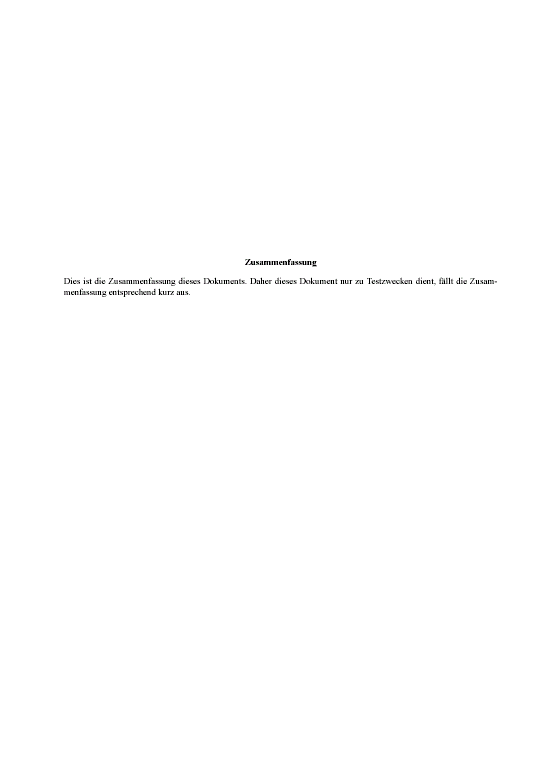
\includegraphics[height=5cm]{images/report_page2.png}}
		\fbox{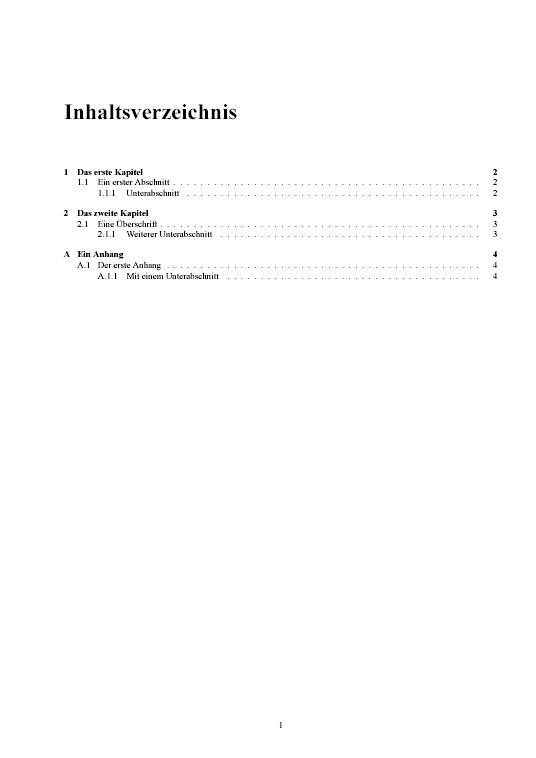
\includegraphics[height=5cm]{images/report_page3.png}} \\
		\fbox{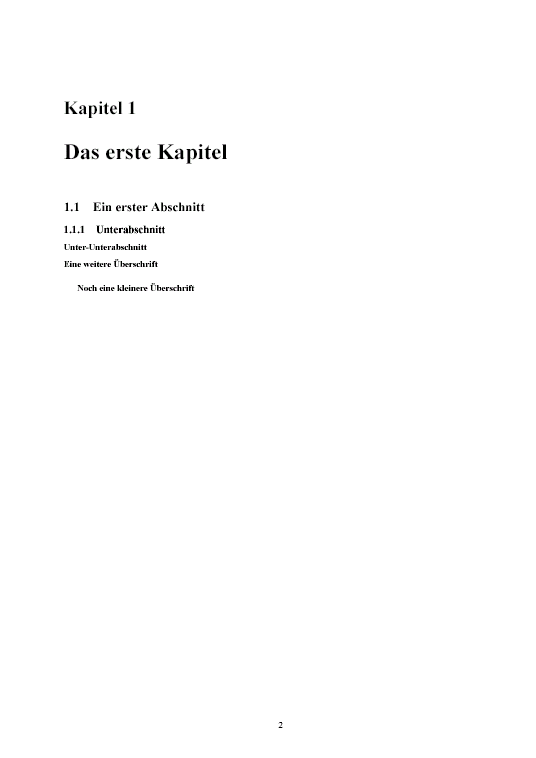
\includegraphics[height=5cm]{images/report_page4.png}}
		\fbox{
\includegraphics[height=5cm]{images/report_page5.png}}
		\fbox{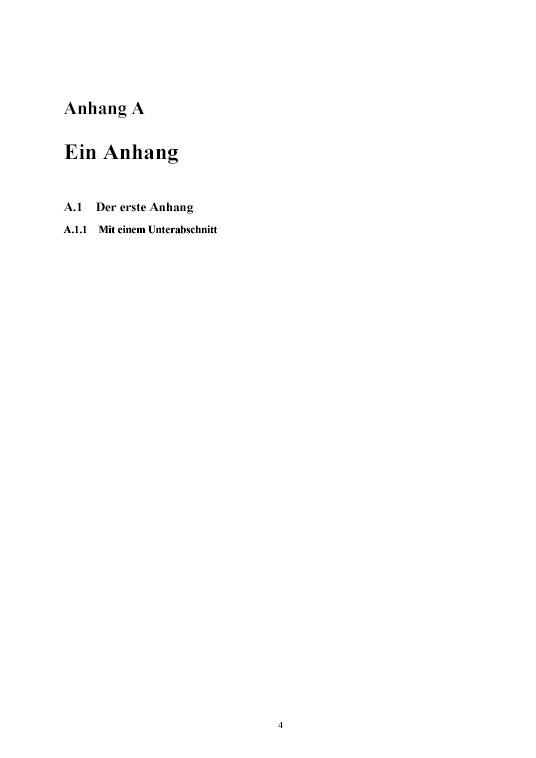
\includegraphics[height=5cm]{images/report_page6.png}}
	\end{center}
	\caption{Aufbau eines Dokuments mit \enquote{scrreprt}}
	\label{fig:report}
\end{figure}


\section{Dokumentklasse \enquote{scrbook}}
\index{Dokumentklasse!scrbook}

\begin{lstlisting}
\documentclass{scrbook}
\end{lstlisting}

Mit der Dokumentklasse \enquote{scrbook} werden die größten Dokumente erstellt. Der Satz ist zweiseitig und die Kapitel beginnen immer auf einer rechten Seite. Natürlich ist der Titel und das Inhaltsverzeichnis auf einer eigenen Seite. In dieser Dokumentklasse existiert keine Zusammenfassung (abstract), da dies bei Büchern unüblich ist. 

Neu hinzu kommt der Befehl \texttt{\textbackslash part}, mit welchem du dein Buch in einzelne Teile unterteilen kannst.

Mögliche Gliederungen in dieser Dokumentklasse sind:
\begin{itemize}
	\item \texttt{\textbackslash part}
	\item \texttt{\textbackslash chapter}
	\item \texttt{\textbackslash section}
	\item \texttt{\textbackslash subsection}
	\item \texttt{\textbackslash subsubsection}
	\item \texttt{\textbackslash paragraph}
	\item \texttt{\textbackslash subparagraph}.
\end{itemize}

\Cref{lst:book} erzeugt neun Seiten, welche du in \cref{fig:book} siehst.

\begin{figure}[htb]
	\begin{center}
		\fbox{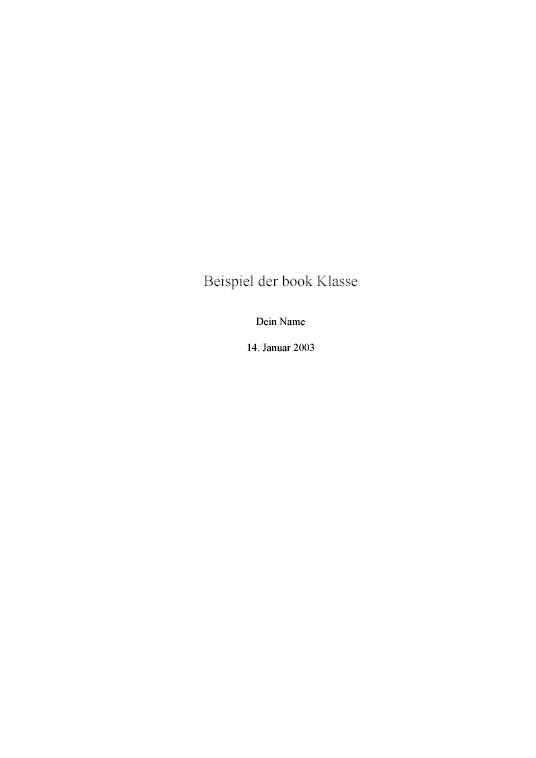
\includegraphics[height=5cm]{images/book_page1.png}}
		\fbox{
\includegraphics[height=5cm]{images/book_page2.png}}
		\fbox{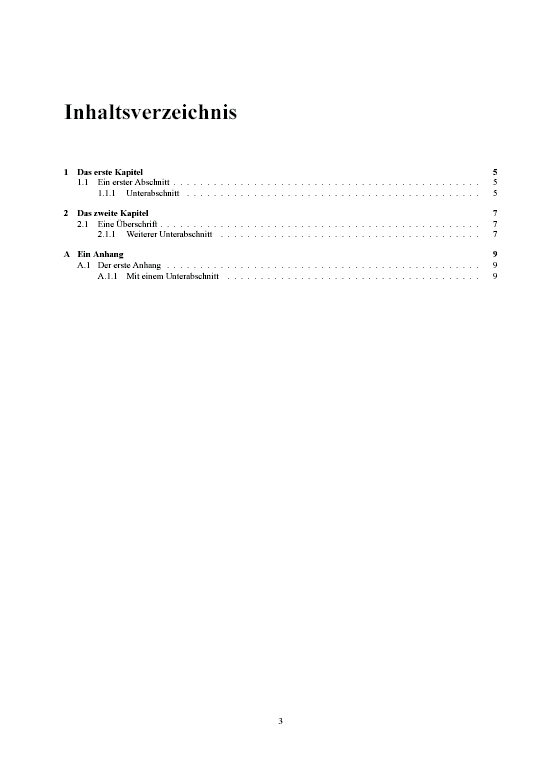
\includegraphics[height=5cm]{images/book_page3.png}} \\
		\fbox{
\includegraphics[height=5cm]{images/book_page4.png}}
		\fbox{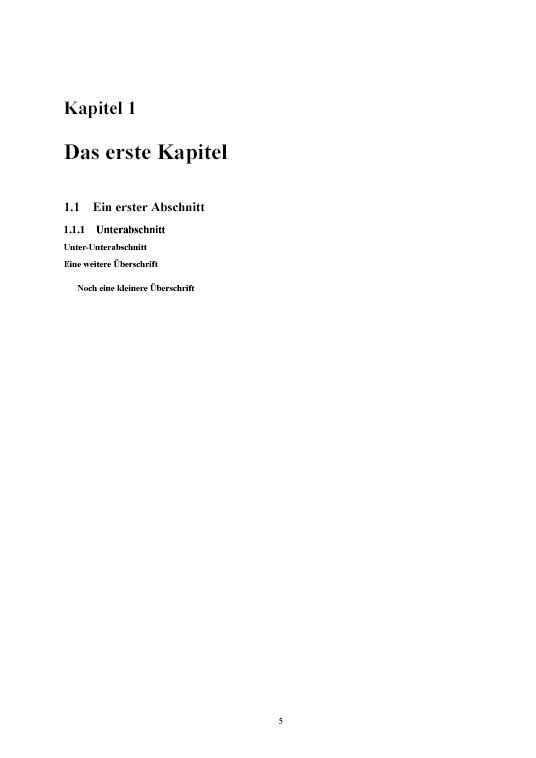
\includegraphics[height=5cm]{images/book_page5.png}}
		\fbox{
\includegraphics[height=5cm]{images/book_page6.png}} \\
		\fbox{
\includegraphics[height=5cm]{images/book_page7.png}}
		\fbox{
\includegraphics[height=5cm]{images/book_page8.png}}
		\fbox{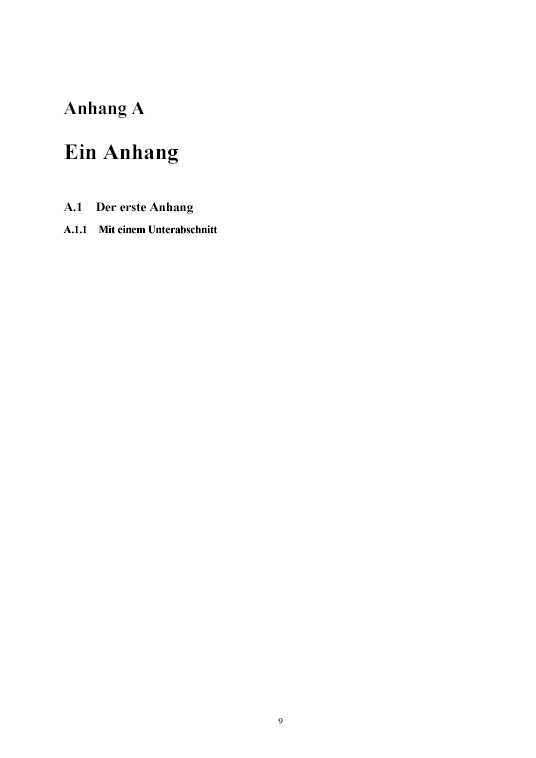
\includegraphics[height=5cm]{images/book_page9.png}}
	\end{center}
	\caption{Aufbau eines Dokuments mit \enquote{scrbook}}
	\label{fig:book}
\end{figure}

%
% EOF
%
